\chapter{Problemspezifikation: Ermittlung eines Lösungsweges}
\label{chap:problemspezifikation}
\minitoc
%%%%%%%%%%%%%%%%%%%%%%%%%%%%%%%%%%%%%%%%%%%%%%%%%%%%%%%
%%%%%%%%%%%%%%%%%%%%%%%%%%%%%%%%%%%%%%%%%%%%%%%%%%%%%%%
%%%%%%%%%%%%%%%%%%%%%%%%%%%%%%%%%%%%%%%%%%%%%%%%%%%%%%%



%%%%%%%%%%%%%%%%%%%%%%%%%%%%%%%%%%%%%%%%%%%%%%%%%%%%%%%
%%%%%%%%%%%%%%%%%%%%%%%%%%%%%%%%%%%%%%%%%%%%%%%%%%%%%%%
%%%%%%%%%%%%%%%%%%%%%%%%%%%%%%%%%%%%%%%%%%%%%%%%%%%%%%%



\section{Anwendung der OOP am Modell}
In der \cref{vkb} wird ein einfaches Energieversorgungsnetz mit vier Knoten
dargestellt. Am Knoten eins ist eine regenerative elektrische Energiequelle, in
diesem Fall ein Windpark, angeschlossen. Weitere konventionelle elektrische
Energiequellen befinden sich an den Knoten zwei und drei. Die passiven Lasten
befinden sich am Knoten zwei und vier. Der Kältespeicher ist am Knoten zwei
angeschlossen. Im Bild wird der Kältespeicher Supermarkt durch einen
Einkaufswagen symbolisiert. Die Knoten sind untereinander durch Leitungen
verbunden.

\begin{figure}[h]
\caption{Vier Knoten Beispiel}
	\label{vkb}
	\begin{center}
	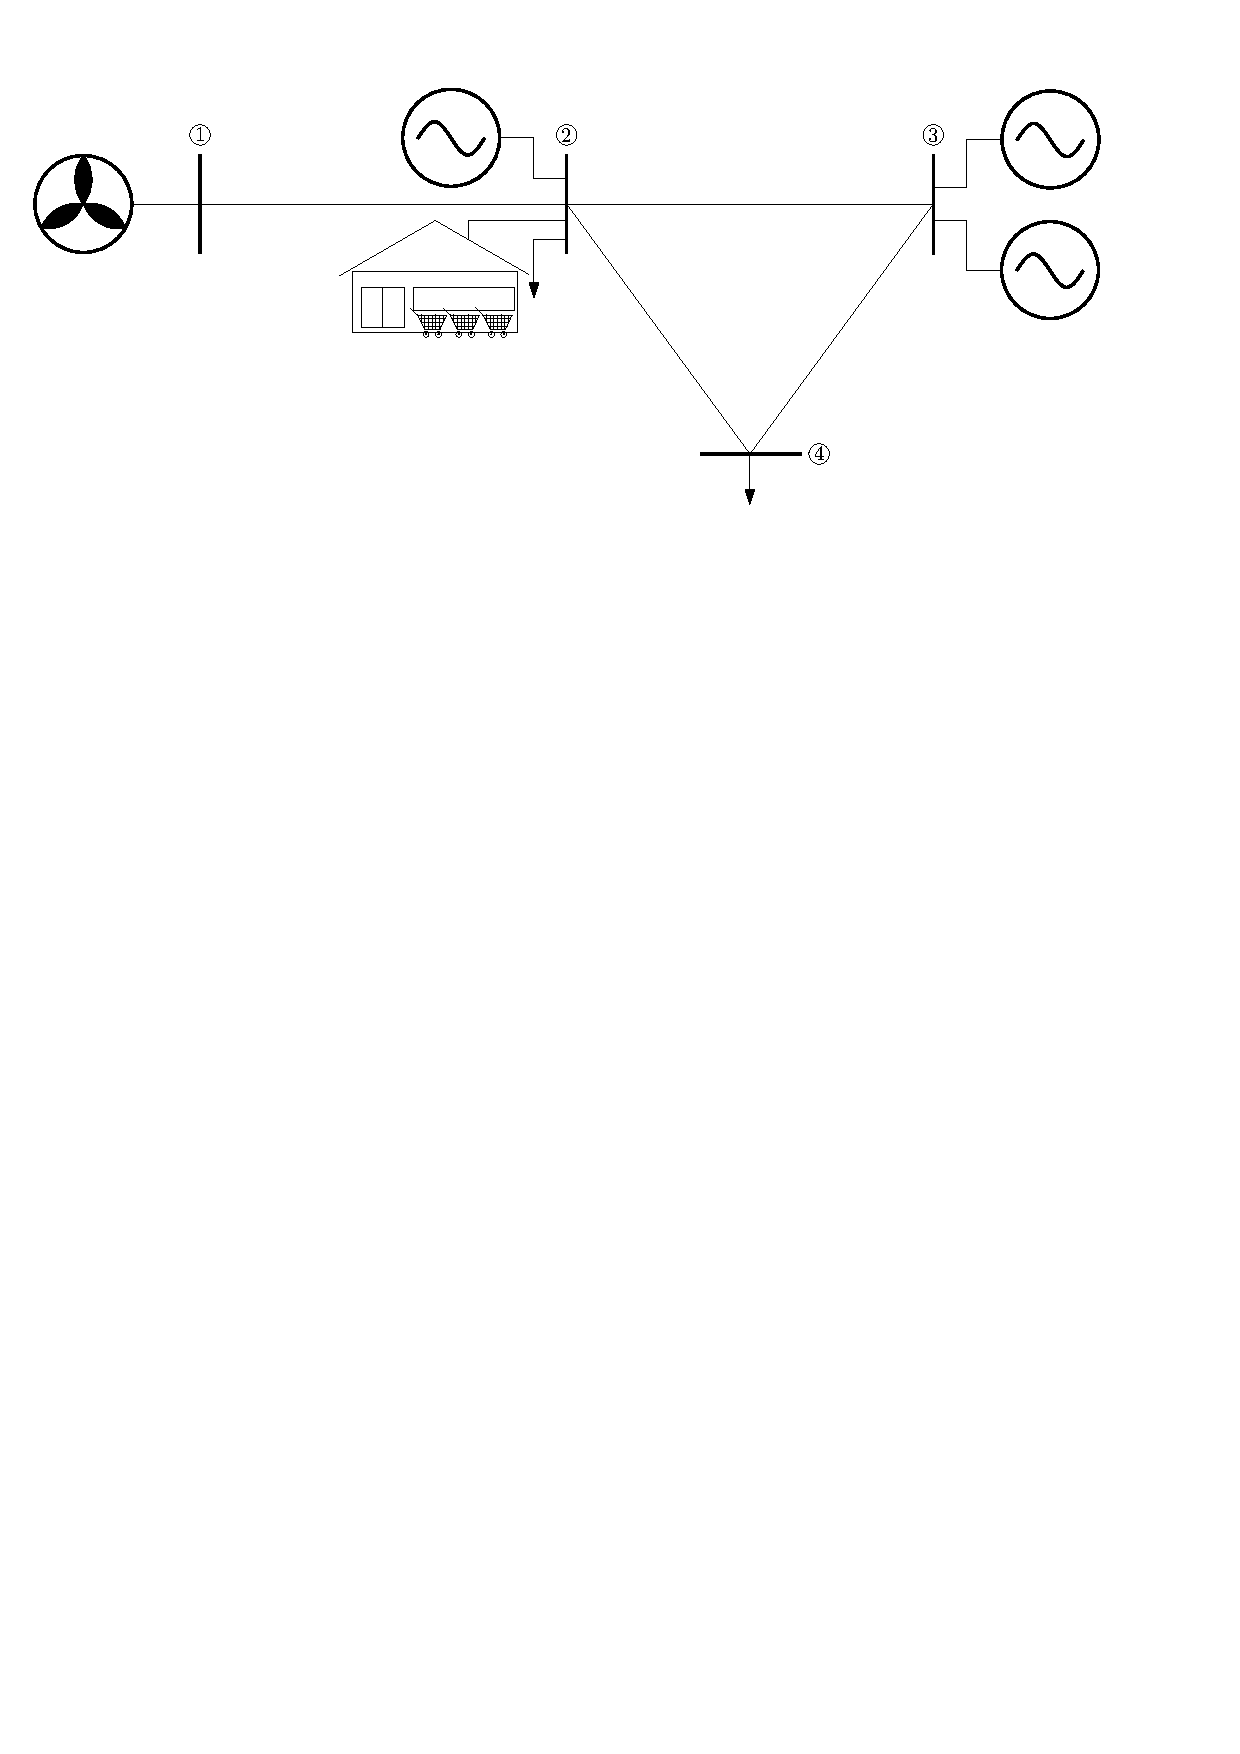
\includegraphics[scale=0.75]{images/SEVN/power_grid}
	\end{center}
\end{figure}

In der Realität kann ein Energieversorgungsnetz durch die Variation der
Knotenzahl und die Vermaschung beliebig komplizierte Form aufweisen. Bei der
Umsetzung der gegebenen Situation im Programm.

\begin{figure}[h]
\caption{Klassendiagramm Modellkonstrukt}
	\label{klassendiagramm}
	\begin{center}
	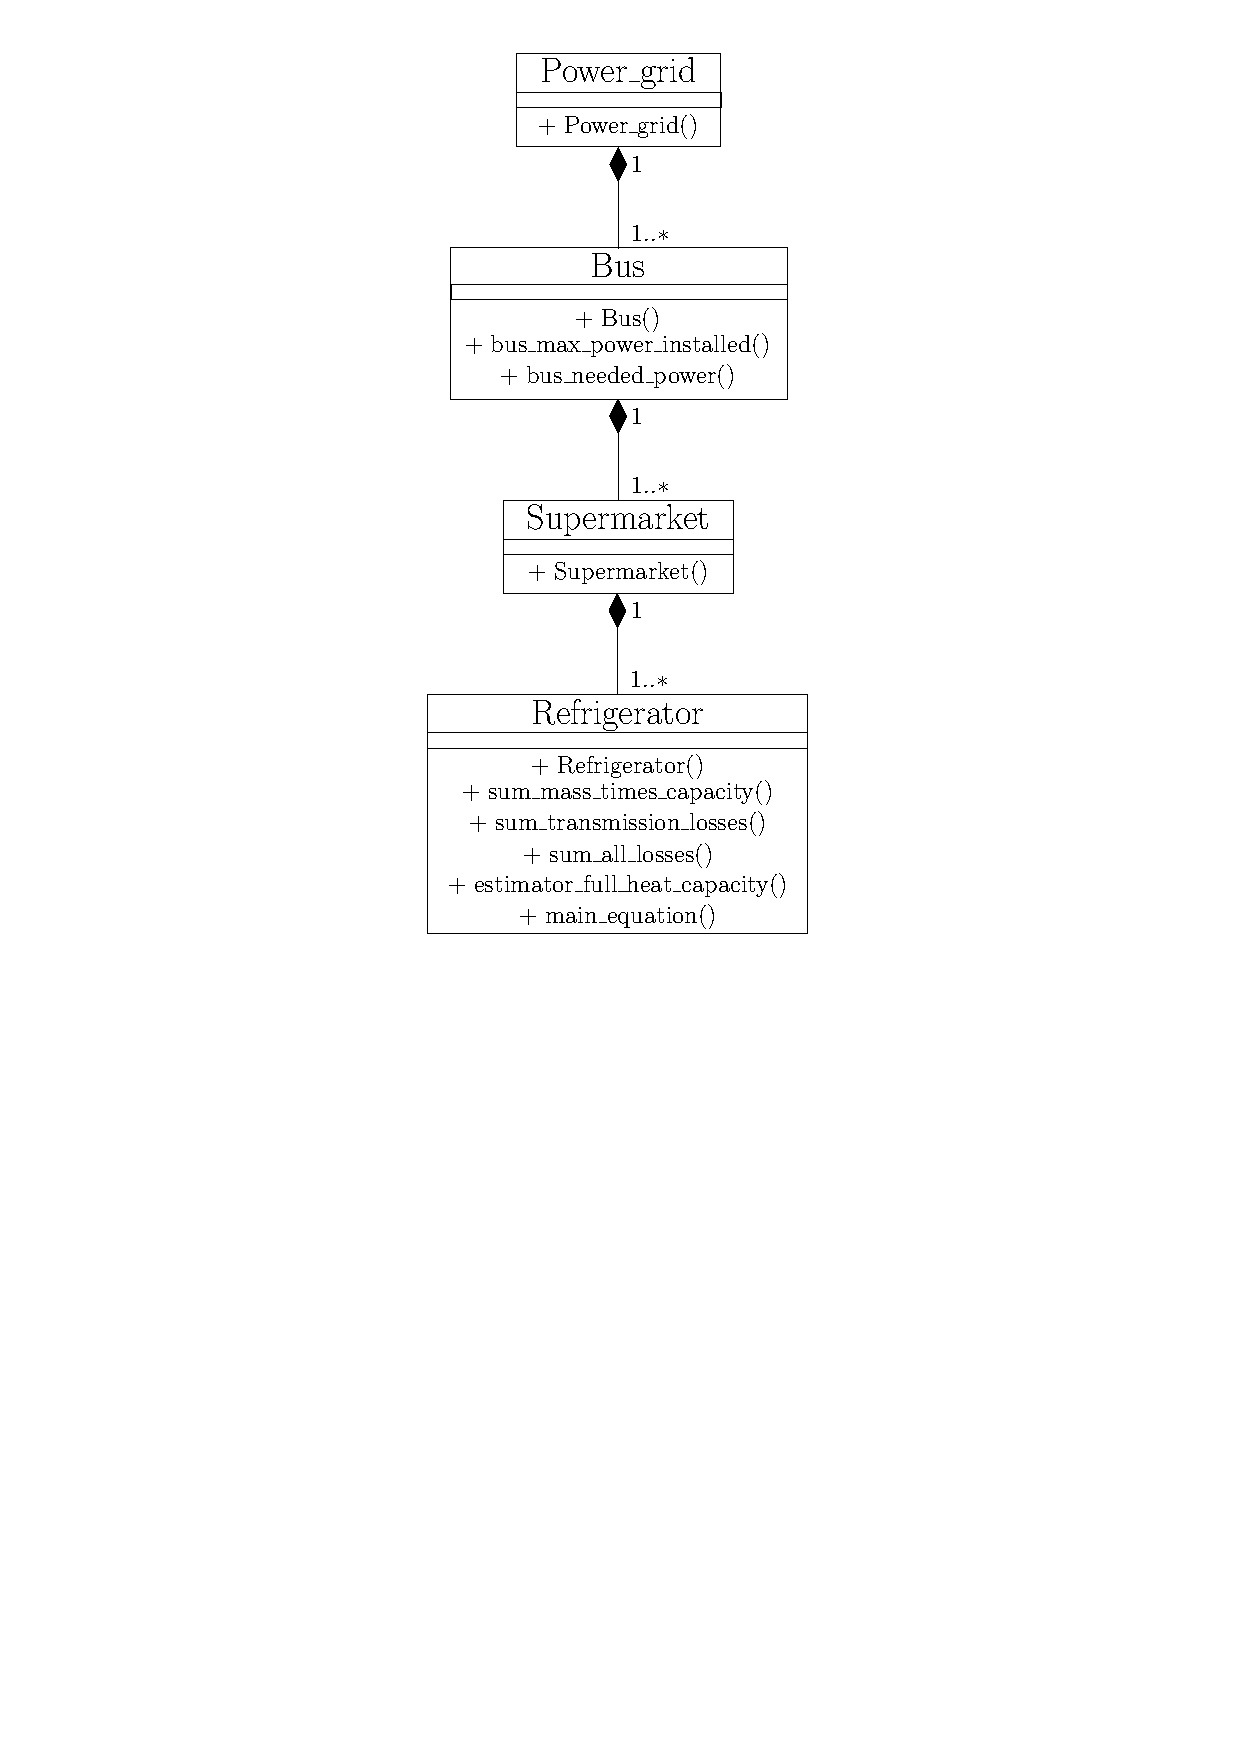
\includegraphics[scale=0.8]{images/Theorie_Super/class_diagramm}
	\end{center}
\end{figure}

Hier noch ein Zwischentext.

\begin{figure}[h]
\caption{Sequenzdiagramm Modellkonstrukt}
	\label{uml_sequence}
	\begin{center}
	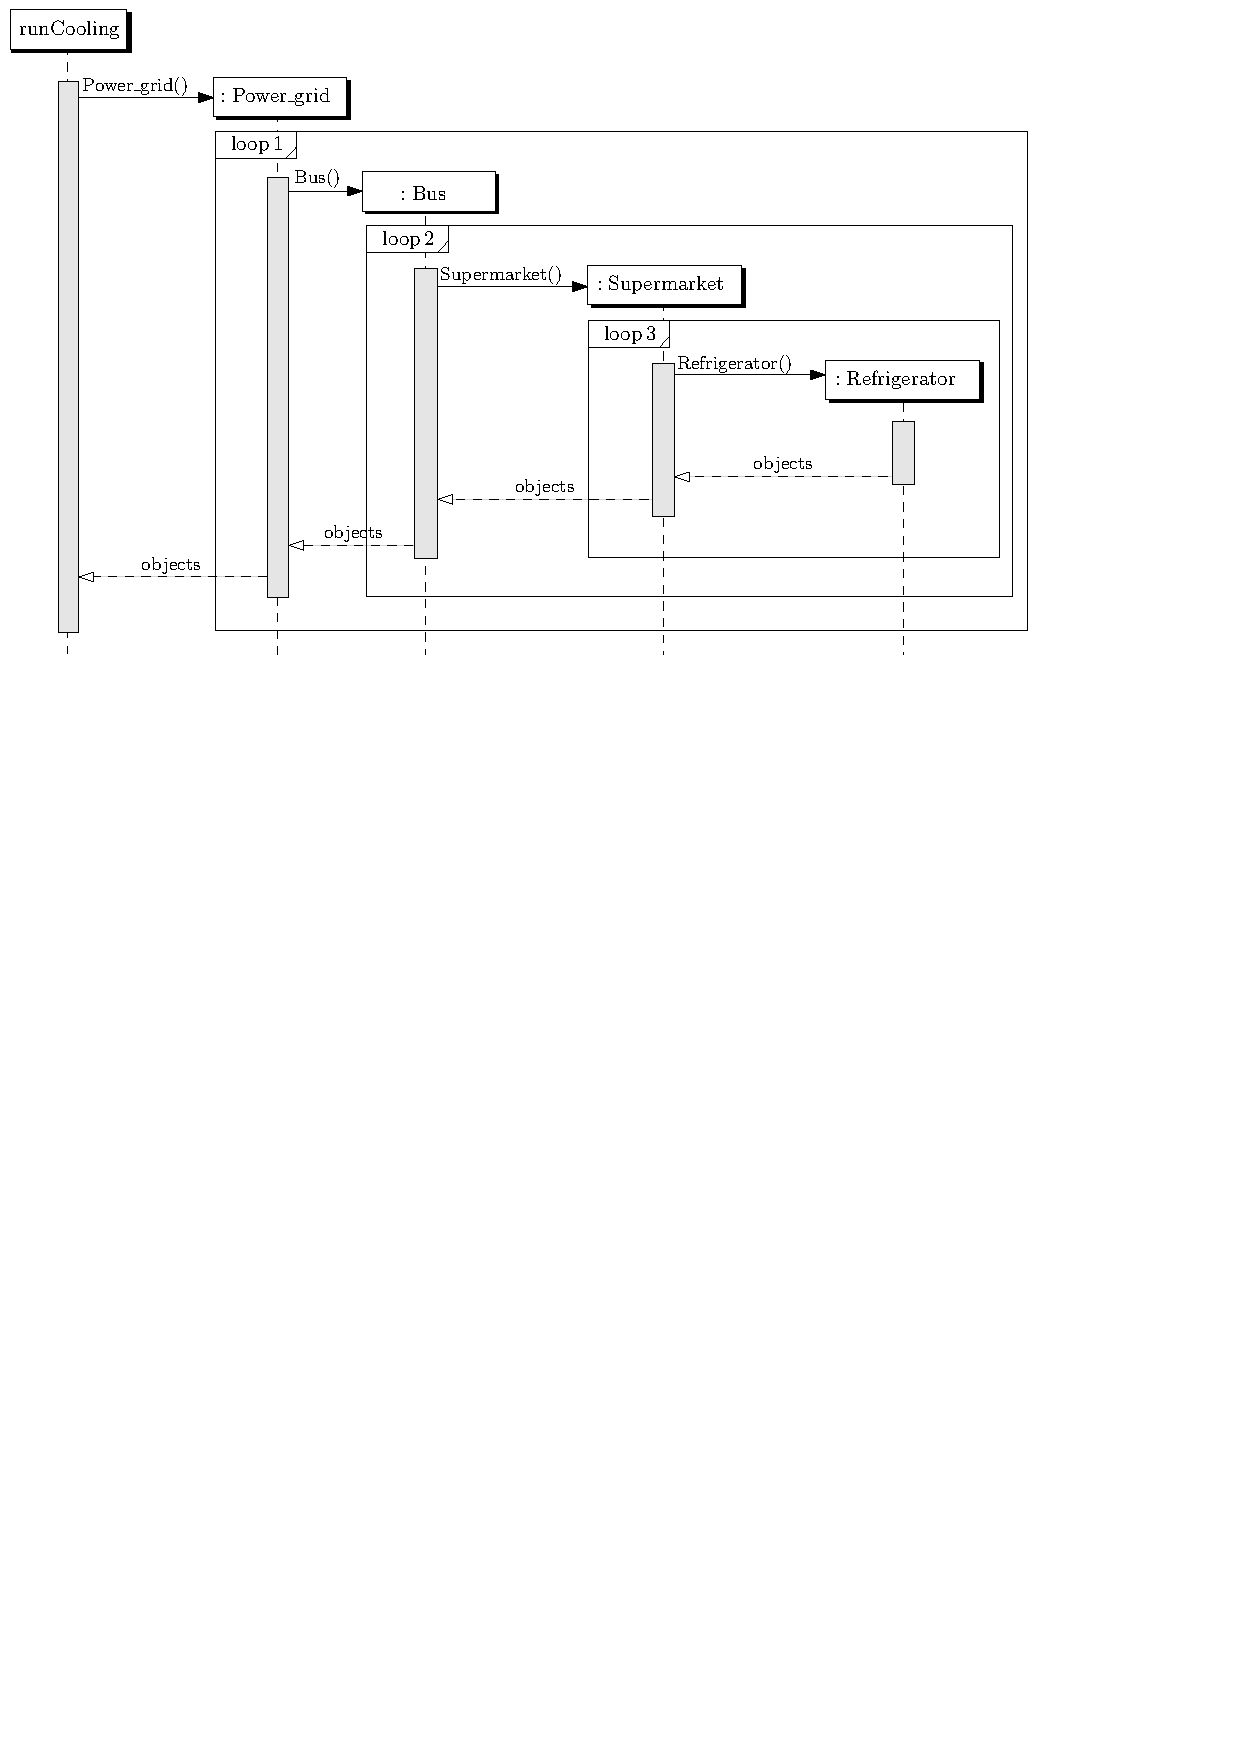
\includegraphics[scale=0.8]{images/Theorie_Super/sequence_one}
	\end{center}
\end{figure}

